\section{Détection d'objet}

\subsection{Blobs d'une image de synthèse}

Nous créons une image binaire de synthèse afin d'en retirer des informations sur les blobs de cette image
grâce à l'objet CBlobResult.

\begin{figure}[H]
      \center
      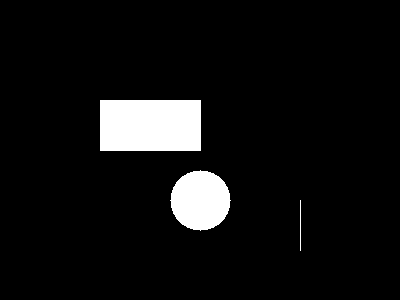
\includegraphics[width=8cm]{ressources/tp5/bin_synth.png}
      \caption{Image synthétique utilisée pour la detection de blobs}
\end{figure}

Nous pouvons voir, lorsque nous affichons les informations de l'image, que la lecture de celle-ci se fait 
de haut en bas et de gauche à droite. Les pixels de l'image sont des pixels carrés et un pixel constitue l'unité atomique d'espace de l'image.
Par conséquent, les caractéristiques du cercle, telles qu'elles sont représentées dans le blob, ne correspondent pas aux caractéristiques théoriques
du cercle qui a été créé dans l'image de synthèse en fournissant son centre et son rayon.\\
%revenir sur la taille du cercle.

Il est possible avec l'objet CBlobResult de filtrer les blobs que l'on souhaite garder. Pour cela,
il faut utiliser la méthode Filter qui prend en paramètre des conditions permettant de sélectionner 
les blobs souhaités. Nous avons par exemple retiré tous les blobs ayant une surface inférieur à 1000 pixels,
ce qui a eu pour conséquence de supprimer le segment de l'objet CBlobResult.
%ajout de l'image et du texte concernant l'affichage des ellipse sur l'image

\subsection{Blobs issus de la détection des doigts}

Nous allons maintenant voir quels sont les réglages optimaux pour obtenir une image binaire des doigts sur 
la vitre en plexiglas. Etant donné que nous travaillons avec des infrarouges, nous avons choisi d'utiliser
le mode couleur IS\_CM\_SENSOR\_RAW8. Nous definissons les autres paramètres avec l'outil uEyeDemo qui nous
fournit un fichier d'initialisation à charger dans notre programme.\\

\begin{figure}[H]
      \center
      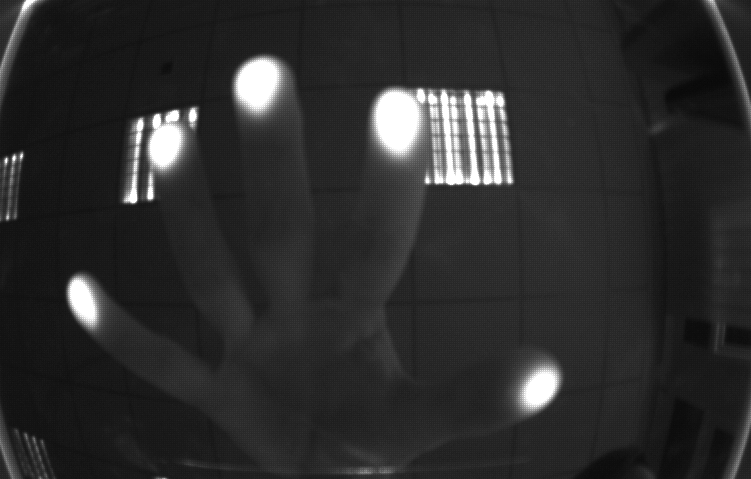
\includegraphics[width=8cm]{ressources/tp5/1-camera_regle_sans_traitement.png}
      \caption{Image de la caméra sans traitement}
\end{figure}

Pour binariser notre image, nous utilisons la méthode d'Otsu. Cependant, nous avons détecté un problème lorsque 
la luminosité du soleil est trop importante à l'acquisition de la première image : toutes les images suivantes sont 
presque totalement blanches. En effet, lorsque la luminosité du soleil est très présente dans l'image, le seuil calculé par
cette méthode est faussé sur les images suivantes. Nous avons donc plutôt utilisé la méthode cvThreshold avec
le paramètre CV\_THRESH\_BINARY et un seuil de 34.\\

\begin{figure}[H]
      \center
      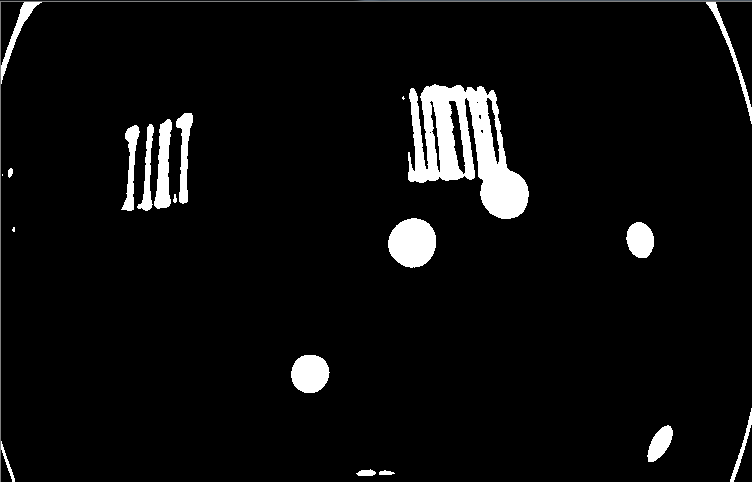
\includegraphics[width=8cm]{ressources/tp5/2-flux_binarise.png}
      \caption{Image de la caméra après binarisation}
\end{figure}

Maintenant que nous avons une image binarisée, nous devons garder seulement les doigts sur l'image. Pour cela, 
nous utilisons la méthode Filter de la classe CBlobResult pour supprimer les néons et autres objets inutiles.
Nous avons utilisé le code suivant :\\
%revoir si on a pas modifié les paramètres
\begin{lstlisting}[caption=Filtrage des blobs via la fonction Filter]
 /* filtre sur l'aire des objets */
 sNewBlobs.Filter(sNewBlobs, B_INCLUDE, CBlobGetArea(), B_INSIDE, 400, 4750);
 /* suppression des formes allonges */
 sNewBlobs.Filter(sNewBlobs, B_INCLUDE, CBlobGetAxisRatio(), B_INSIDE, 0.5, 1);
 /* suppression des objets non compacte */
 sNewBlobs.Filter(sNewBlobs, B_EXCLUDE, CBlobGetCompactness(), B_GREATER, 5.0);
\end{lstlisting}
%mettre image avant modifiation

%12 horloge pixel
%26.15 cadence
%7 temp d'integration

%binarisation avec otsu -> probleme quand il y a du soleil

%modification du filtre des blobs
%	- taille entre 400 et 4400
%	- ratio entre 
\subsection{Etiquetage des blobs}

Pour pouvoir identifier chaque doigt sur l'image, nous devons passer sur une image couleur via la fonction cvMerge.
Puis, via un tableau de couleurs nous faisons correspondre une couleur à un numéro de blob du CBlobResult, ce qui nous donne
le résultat suivant.\\

\begin{figure}[H]
      \center
      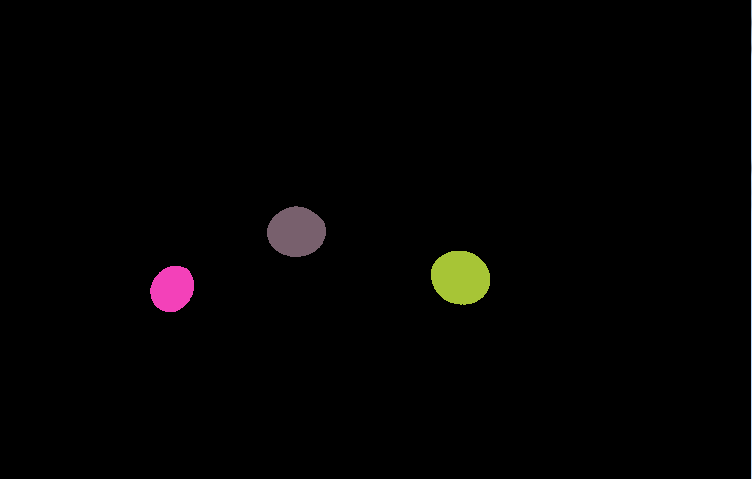
\includegraphics[width=8cm]{ressources/tp5/3-flux_indexe.png}
      \caption{Image de la caméra après indexage}
\end{figure}

Le problème avec cette méthode c'est qu'avec le sens de lecture des blobs, il est possible que lorsque nous effectuons 
une rotation avec deux doigts sur la plaque de plexiglas, les couleurs des doigts changent durant le mouvement.
Puisque la première couleur est utilisée pour le premier blob, si l'image lit le deuxième doigt en premier alors sa couleur
change, le sens de lecture étant de gauche à droite et de haut en bas.
